\documentclass[11pt,a4paper]{article}
\usepackage{gtu-el-yazisi}
\begin{document}
\notbilgi{İşaretler ve Sistemler}{Ders 4 -- LTI sistemlerin özellikleri, birim basamak cevabı}{Isaret-ve-Sistemler-ders-4.pdf}
\renewcommand{\thempfootnote}{\alph{mpfootnote}} % kutu içi dipnotlar için (euler + \itshape uyumsuzluğu)

\subsection{3) Nedensel ve nedensel olmayan LTI sistemler}
\sayfa{1}
(Causal and noncausal LTI systems)

Reminder: Bir sistemin herhangi bir zamandaki çıktısı girdinin gelecek değerlerine bağlı değilse nedenseldir.
\begin{align*}
  y[n] = x[n] \ast h[n] &= \sum_{k=-\infty}^{\infty} x[k]\,h[n-k] = \sum_{k=-\infty}^{\infty} h[k]\,x[n-k] \\
  &= \cdots + h[0]\,x[n] + \underbrace{h[-1]\,x[n+1] + h[-2]\,x[n+2] + \cdots}_{\substack{\text{Nedensel olması için}\\ n<0 \text{ iken } h[n]=0 \text{ olmalı}}}
\end{align*}

\begin{align*}
  \text{Nedensel: } & h[n] = 0, \ n < 0 \\
  & y[n] = \sum_{k=-\infty}^{n} x[k]\,h[n-k] = \sum_{k=0}^{\infty} h[k]\,x[n-k]
\end{align*}

$\Rightarrow$ Bir LTI sistem nedensel ise, bu sistemin dürtü cevabı dürtü uygulanmadan önce sıfır olmalıdır.
\begin{align*}
  & h(t) = 0, \ t < 0 \\
  & y(t) = \int_{-\infty}^{t} x(\tau)\,h(t-\tau)\,d\tau = \int_{0}^{\infty} h(\tau)\,x(t-\tau)\,d\tau
\end{align*}

\subsection{4) Kararlı ve kararlı olmayan LTI sistemler}
(Stable and nonstable LTI systems)

Reminder: \ $|x(t)| \leq M_x < \infty \longrightarrow |y(t)| \leq M_y < \infty$ \ ise kararlıdır.
\begin{gather*}
  |x[n]| \leq M_x < \infty, \ \forall n \\
  |y[n]| = \left|\sum_{k=-\infty}^{\infty} h[k]\,x[n-k]\right| \leq \sum_{k=-\infty}^{\infty} |h[k]|\,|x[n-k]| \leq M_x \underbrace{\sum_{k=-\infty}^{\infty} |h[k]|}_{<\infty \text{ olmalı}}, \quad \forall n
\end{gather*}
\begin{align*}
  \text{Kararlı: } & \sum_{k=-\infty}^{\infty} |h[k]| < \infty \\
  & \int_{-\infty}^{\infty} |h(\tau)|\,d\tau < \infty
\end{align*}

\begin{ornek}[(Ex)]
$y[n] = \displaystyle\sum_{k=-\infty}^{n} x[k]$ \ kararlı mıdır? \hfill \fcolorbox{kirmizikalem}{kagitrengi}{\parbox{2.4cm}{\color{turuncukalem}\small u[n-k]\\ n-k>0\\ n>k}}
\begin{align*}
  & y[n] = x[n] \ast h[n] = \sum_{k=-\infty}^{\infty} x[k]\,h[n-k] \longleftarrow h[n] = u[n] \\
  & \sum_{k=-\infty}^{\infty} |h[k]| = \sum_{k=-\infty}^{\infty} |u[k]| = \sum_{k=0}^{\infty} u[k] \to \infty \quad \text{Kararsızdır.}
\end{align*}
\end{ornek}

\begin{ornek}[(Ex)]
$h(t) = \delta(t-t_0)$
\[ \int_{-\infty}^{\infty} |\delta(t-t_0)|\,dt = 1 < \infty \quad \text{Kararlı} \]
\end{ornek}

\subsection{Birim basamak cevabı (unit step response):}
Bir LTI sistemin birim basamak cevabı $s[n]\,/\,s(t)$, sisteme birim basamak işareti $u[n]\,/\,u(t)$ uygulandığında elde edilen çıktıdır.
\begin{center}
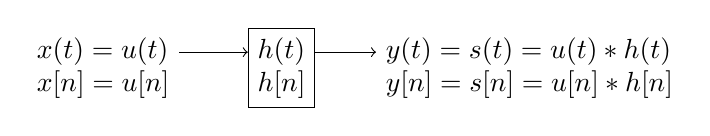
\begin{tikzpicture}
  \node[draw, align=left, minimum height=0.9cm] (H) at (0,0) {$h(t)$\\ $h[n]$};
  \node[left, align=left] at (-1.3,0) {$x(t) = u(t)$\\ $x[n] = u[n]$};
  \draw[->] (-1.3,0.2) -- (H.west |- 0,0.2);
  \draw[->] (H.east |- 0,0.2) -- (1.2,0.2);
  \node[right, align=left] at (1.2,0) {$y(t) = s(t) = u(t) \ast h(t)$\\ $y[n] = s[n] = u[n] \ast h[n]$};
\end{tikzpicture}
\end{center}
\begin{gather*}
  s(t) = u(t) \ast h(t) = \int_{-\infty}^{\infty} h(\tau)\,u(t-\tau)\,d\tau = \int_{-\infty}^{t} h(\tau)\,d\tau \longrightarrow h(t) = \frac{ds(t)}{dt} = s'(t) \\
  s[n] = u[n] \ast h[n] = \sum_{k=-\infty}^{n} h[k] \longrightarrow h[n] = s[n] - s[n-1]
\end{gather*}

\section{Nedensel LTI Sistemlerin Türev/Fark Denklemleri ile Tanımlanması:}
\sayfa{2}
Sürekli zamanlı nedensel LTI sistemler lineer sabit katsayılı türev denklemleri ile ifade edilebilir.
\begin{itemize}[label=--]
  \item RC devresi
\end{itemize}
Ayrık zamanlı nedensel LTI sistemler lineer sabit katsayılı fark denklemleri ile ifade edilebilir.
\begin{itemize}[label=--]
  \item Farklı prosedürlerin sıralı davranışları
\end{itemize}

\subsection{Lineer sabit katsayılı Türev denklemleri:}
(Linear constant-coefficient differential equations)

\[ \sum_{k=0}^{N} a_k\,\frac{d^k y(t)}{dt^k} = \sum_{k=0}^{M} b_k\,\frac{d^k x(t)}{dt^k} \quad : \ \text{Nth-order linear constant-coeff. diff. eq.} \]
Order (mertebe): Çıkış işareti $y(t)$'nin en yüksek türevinin derecesidir.
\begin{align*}
  N = 0 \ &\Rightarrow\ y(t) = \frac{1}{a_0}\sum_{k=0}^{M} b_k\,\frac{d^k x(t)}{dt^k} \\
  N \geq 1 \ &\Rightarrow\ y(t) = y_p(t) + y_h(t)
\end{align*}
\begin{itemize}[label={}, leftmargin=1.5em]
  \item $y_p(t)$: özel çözüm (particular solution) giriş işaretine bağlı olarak elde edilir
  \item $y_h(t)$: homojen çözüm (homogeneous solution) başlangıç değerlerine (initial conditions) göre elde edilir.\\
  \phantom{$y_h(t)$: }Doğal çözüm (natural response)
\end{itemize}
\[ \sum_{k=0}^{N} a_k\,\frac{d^k y(t)}{dt^k} = 0 \ : \ \text{Homojen çözüm için bu eşitliğin çözülmesi gerekir.} \]

Nedensel LTI sistemlerin durgun olma koşulu (giriş sıfır olduğu süre çıkışta sıfırdır) kullanılarak giriş ve çıkışın sıfırdan farklı olduğu ilk zaman başlangıç noktası olarak alınır.
\begin{gather*}
  x(t) = 0, \ t \leq t_0 \ \text{ iken } \ y(t) = 0, \ t \leq t_0 \\
  y(t_0) = \frac{dy(t_0)}{dt} = \frac{d^2 y(t_0)}{dt^2} = \cdots = \frac{d^{N-1} y(t_0)}{dt^{N-1}} = 0
\end{gather*}

\begin{ornek}[(Ex)]
$\dfrac{dy(t)}{dt} + 2y(t) = x(t)$, \quad $x(t) = K e^{3t}u(t)$, \quad $y(t) = ?$
\end{ornek}
\begin{cozum}
\[ y(t) = \underset{\substack{\downarrow\\ \text{özel çözüm (girişe bağlı)}}}{y_p(t)} + \underset{\substack{\downarrow\\ \text{homojen/doğal çözüm (başlangıç koşullarına bağlı)}}}{y_h(t)} \]

$\Rightarrow$ Özel çözüm \ $y_p(t) = Y e^{3t}u(t)$ \ yada \ $y_p(t) = Y e^{3t}$, $t > 0$ \ olarak seçilir.

Not: Üstel formlu bir giriş işareti için özel çözüm yine üstel formlu bir işarettir.
\[ 3Y e^{3t} + 2Y e^{3t} = K e^{3t} \longrightarrow 5Y = K \rightarrow Y = \frac{K}{5} \quad \Longleftarrow \ \frac{dy(t)}{dt} + 2y(t) = x(t) \]
\[ y_p(t) = \frac{K}{5}\,e^{3t}u(t) \]

\sayfa{3}
$\Rightarrow$ Homojen çözüm \ $y_h(t) = A e^{st}$ \ olarak seçilir.
\[ A s e^{st} + 2A e^{st} = 0 \longrightarrow A e^{st}(s+2) = 0 \longrightarrow s = -2 \quad \Longleftarrow \ \frac{dy(t)}{dt} + 2y(t) = 0 \]
\[ y_h(t) = A e^{-2t} \]
$A = ?$ $\rightarrow$ Durgun olma koşulu / başlangıç değerinden bulunur.

$t > 0$ için tanımlı

$x(t) = 0$, $t \leq 0$ iken $y(t) = 0$, $t \leq 0$ ise $y(0) = 0$

$\Rightarrow$ Genel çözüm \ $y(t) = y_p(t) + y_h(t) = \dfrac{K}{5}e^{3t} + A e^{-2t}$, \ $t > 0$
\[ y(0) = \frac{K}{5} + A = 0 \ \Rightarrow\ A = -\frac{K}{5} \]
\[ y(t) = \frac{K}{5}\bigl[e^{3t} - e^{-2t}\bigr]\,u(t) \quad \text{yada} \quad y(t) = \begin{cases} \dfrac{K}{5}\bigl[e^{3t} - e^{-2t}\bigr], & t > 0 \\[2mm] 0, & t \leq 0 \end{cases} \]
\end{cozum}

\subsection{Lineer sabit katsayılı fark denklemleri:}
(Linear constant-coefficient difference equations)

\[ \sum_{k=0}^{N} a_k\,y[n-k] = \sum_{k=0}^{M} b_k\,x[n-k] \ : \ \text{Nth-order linear const.-coeff. difference eq.} \qquad \tikz[baseline=(c.base)]\node[draw,circle,inner sep=1pt](c){\small 1}; \]
\[ y[n] = \underset{\substack{\downarrow\\ \text{özel çözüm}}}{y_p[n]} + \underset{\substack{\downarrow\\ \text{homojen çözüm}}}{y_h[n]} \qquad \sum_{k=0}^{N} a_k\,y[n-k] = 0 \]
Başlangıç koşulları (nedensel LTI durağanlık koşulu): \ $x[n] = 0$, $n < n_0$ ise \ $y[n] = 0$, $n < n_0$
\[ y[n] = \frac{1}{a_0}\left[\sum_{k=0}^{M} b_k\,x[n-k] - \sum_{k=1}^{N} a_k\,y[n-k]\right] \qquad \tikz[baseline=(c.base)]\node[draw,circle,inner sep=1pt](c){\small 2}; \]
\tikz[baseline=(c.base)]\node[draw,circle,inner sep=1pt](c){\small 1}; ve \tikz[baseline=(c.base)]\node[draw,circle,inner sep=1pt](c){\small 2}; bağıntıları özyinelemeli (recursive) ifadelerdir ($n$. andaki çıkış, kendinden önceki çıkış değerlerine bağlı olduğundan)

$\Rightarrow$ $N = 0$ iken
\[ y[n] = \sum_{k=0}^{M} \frac{b_k}{a_0}\,x[n-k] \ : \ \text{non-recursive} \]
($y[n]$ doğrudan giriş ve girişin önceki değerlerinden hesaplanabilir, kendinin önceki değerlerine `başlangıç koşullarına' ihtiyaç duymaz)

\noindent
\begin{minipage}[c]{0.4\linewidth}
Dürtü cevabı (impulse response)
\[ h[n] = \begin{cases} \dfrac{b_n}{a_0}, & 0 \leq n \leq M \\[2mm] 0, & \text{dışında} \end{cases} \]
\end{minipage}\hfill
\begin{minipage}[c]{0.58\linewidth}
\[ \Longleftarrow \ y[n] = x[n] \ast h[n] = \sum_{-\infty}^{\infty} h[k]\,x[n-k] \]
\end{minipage}

$N = 0$ iken elde edilen dürtü cevabı sonlu bir zaman aralığında sıfırdan farklı olduğundan
$y[n] = \sum_{k=0}^{M} \frac{b_k}{a_0}\,x[n-k]$ sistemi sonlu dürtü tepkili (finite impulse response, FIR) olarak isimlendirilir.

$\Rightarrow$ $N \geq 1$ için \ $y[n] = \dfrac{1}{a_0}\left[\displaystyle\sum_{k=0}^{M} b_k\,x[n-k] - \sum_{k=1}^{N} a_k\,y[n-k]\right]$ \ fark denklemi ile verilen sistemin
\sayfa{4}
çözümü $y[n] = y_p[n] + y_h[n]$ şeklinde elde edilir ve başlangıç değerlerine ihtiyaç duyar.
Bu sistemin dürtü cevabı sonsuz zaman aralığında sıfırdan farklı olduğundan, sistem sonsuz dürtü tepkili (infinite impulse response, IIR) olarak isimlendirilir.

\begin{ornek}[(Ex)]
$y[n] - \frac{1}{2}y[n-1] = x[n]$, \quad $x[n] = K\delta[n]$, \quad $y[n] = ?$
\end{ornek}
\begin{cozum}
\[ y[n] = x[n] + \frac{1}{2}y[n-1] \quad \longleftarrow \ x[n] = 0, \ n \leq -1 \ \text{ iken } \ y[n] = 0, \ n \leq -1 \]
\begin{align*}
  y[-1] &= x[-1] + \tfrac{1}{2}y[-2] = 0 \\
  y[0] &= x[0] + \tfrac{1}{2}y[-1] = K\underset{\swarrow 1}{\delta[0]} + \tfrac{1}{2}\underset{\swarrow 0}{y[-1]} = K \\
  y[1] &= \underset{\swarrow 0}{x[1]} + \tfrac{1}{2}y[0] = \tfrac{1}{2}K \\
  y[2] &= x[2] + \tfrac{1}{2}y[1] = \left(\tfrac{1}{2}\right)^2 K \\
  y[3] &= x[3] + \tfrac{1}{2}y[2] = \left(\tfrac{1}{2}\right)^3 K \\
  &\ \vdots \\
  y[n] &= x[n] + \tfrac{1}{2}y[n-1] = \left(\tfrac{1}{2}\right)^n K
\end{align*}
\[ h[n] = \left(\frac{1}{2}\right)^n u[n], \quad K = 1 \ \text{iken} \quad (\text{IIR}) \]
\end{cozum}

$\Rightarrow$ Birinci dereceden fark denklemi ile tanımlanmış sistemlerin blok diyagramı ile gösterilimi
\begin{center}
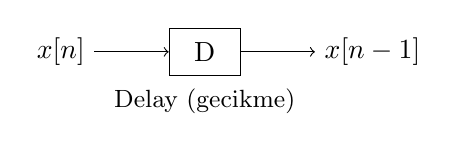
\begin{tikzpicture}
  \node[draw, minimum width=0.9cm, minimum height=0.6cm] (D) at (0,0) {D};
  \draw[->] (-1.4,0) node[left] {$x[n]$} -- (D.west);
  \draw[->] (D.east) -- (1.4,0) node[right] {$x[n-1]$};
  \node[below] at (0,-0.35) {\small Delay (gecikme)};
\end{tikzpicture}
\end{center}
Gecikme, bellek elemanına karşılık gelir, ve girişin bir önceki değerini tutar. Nedensel LTI sistemlerde olduğu gibi durağan olma koşulu uygulanırsa bellek elemanında depolanan başlangıç değeri sıfırdır.

\noindent
\begin{minipage}[c]{0.4\linewidth}
\begin{align*}
  & y[n] + a\,y[n-1] = b\,x[n] \\
  \hookrightarrow\ & y[n] = b\,x[n] - a\,y[n-1]
\end{align*}
\end{minipage}\hfill
\begin{minipage}[c]{0.56\linewidth}
\centering
\begin{tikzpicture}
  \node[draw, circle, inner sep=0pt, minimum size=0.32cm] (S) at (0,0) {$+$};
  \draw[->] (-1.4,0) node[left] {$x[n]$} -- node[above] {$b$} (S.west);
  \draw[->] (S.east) -- (3,0) node[right] {$y[n]$};
  \node[draw, minimum width=0.7cm, minimum height=0.6cm] (D) at (1.8,-1.1) {D};
  \draw[->] (1.8,0) -- (D.north);
  \draw[->] (D.south) |- node[pos=0.25, right] {$y[n-1]$} node[pos=0.75, below] {$-a$} (0,-2.2) -- (S.south);
\end{tikzpicture}
\end{minipage}

$\Rightarrow$ Birinci dereceden türev denklemi ile tanımlanmış sistemlerin blok diyagramı ile gösterilimi
\sayfa{5}
\[ \frac{dy(t)}{dt} + a\,y(t) = b\,x(t) \]
\begin{center}
\begin{tikzpicture}
  \node[draw, minimum width=0.9cm, minimum height=0.6cm] (D) at (0,0) {D};
  \draw[->] (-1.4,0) node[left] {$x(t)$} -- (D.west);
  \draw[->] (D.east) -- (1.2,0) node[right] {$\dfrac{dx(t)}{dt}$};
  \node[below, align=center] at (0,-0.4) {\small differentiator\\ \small (Türev alıcı)};
\end{tikzpicture}
\end{center}

\noindent
\begin{minipage}[c]{0.4\linewidth}
\[ y(t) = \frac{b}{a}\,x(t) - \frac{1}{a}\,\frac{dy(t)}{dt} \]
\end{minipage}\hfill
\begin{minipage}[c]{0.56\linewidth}
\centering
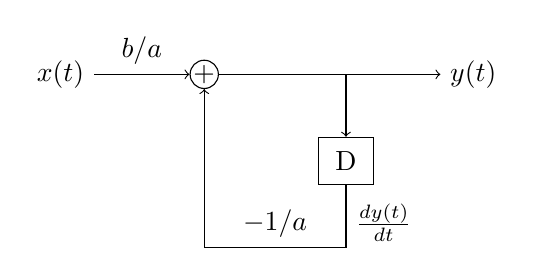
\begin{tikzpicture}
  \node[draw, circle, inner sep=0pt, minimum size=0.32cm] (S) at (0,0) {$+$};
  \draw[->] (-1.4,0) node[left] {$x(t)$} -- node[above] {$b/a$} (S.west);
  \draw[->] (S.east) -- (3,0) node[right] {$y(t)$};
  \node[draw, minimum width=0.7cm, minimum height=0.6cm] (D) at (1.8,-1.1) {D};
  \draw[->] (1.8,0) -- (D.north);
  \draw[->] (D.south) |- node[pos=0.3, right] {$\frac{dy(t)}{dt}$} node[pos=0.75, above] {$-1/a$} (0,-2.2) -- (S.south);
\end{tikzpicture}
\end{minipage}

Türev alıcıların pratik gerçeklemesi zor olduğundan alternatif bir gösterilime gidilir:
\[ \frac{dy(t)}{dt} = b\,x(t) - a\,y(t) \longrightarrow y(t) = \int_{-\infty}^{t} \bigl[b\,x(\tau) - a\,y(\tau)\bigr]\,d\tau \]
\begin{center}
\begin{tikzpicture}
  \node[draw, circle, inner sep=0pt, minimum size=0.32cm] (S) at (0,0) {$+$};
  \node[draw, minimum width=0.8cm, minimum height=0.7cm] (I) at (1.3,0) {$\int$};
  \draw[->] (-1.4,0) node[left] {$x(t)$} -- node[above] {$b$} (S.west);
  \draw[->] (S.east) -- (I.west);
  \draw[->] (I.east) -- (3.4,0) node[right] {$y(t)$};
  \draw[->] (2.7,0) |- node[pos=0.75, below] {$-a$} (0,-1.1) -- (S.south);
\end{tikzpicture}
\end{center}
\[ y(t) = y(t_0) + \int_{t_0}^{t} \bigl[b\,x(\tau) - a\,y(\tau)\bigr]\,d\tau \]
Burada, integral alıcı $y(t_0)$'daki başlangıç değerini belleğinde tutar.

\begin{ornek}[(Ex)]
$y[n] - \frac{1}{2}y[n-1] = x[n]$, \quad $x[n] = \left(\frac{1}{3}\right)^n u[n]$, \quad $y[n] = ?$
\end{ornek}
\begin{cozum}
\[ y[n] = y_p[n] + y_h[n] \]
$y_p[n] = A\left(\frac{1}{3}\right)^n u[n]$ olsun.
\begin{gather*}
  A\left(\tfrac{1}{3}\right)^n - \tfrac{1}{2}A\left(\tfrac{1}{3}\right)^{n-1} = \left(\tfrac{1}{3}\right)^n \ \rightarrow\ A - \frac{3A}{2} = 1 \ \rightarrow\ A = -2 \\
  y_p[n] = -2\left(\tfrac{1}{3}\right)^n, \quad n \geq 0
\end{gather*}
$y_h[n] = B\alpha^n$ olsun. \ $y[n] - y[n-1] = 0$\footnotemark
\begin{gather*}
  B\alpha^n - \tfrac{1}{2}B\alpha^{n-1} = 0 \ \rightarrow\ \alpha = \tfrac{1}{2} \\
  y_h[n] = B\left(\tfrac{1}{2}\right)^n
\end{gather*}
\[ y[n] = -2\left(\tfrac{1}{3}\right)^n + B\left(\tfrac{1}{2}\right)^n, \ n \geq 0 \qquad y[0] = 1 \ \longleftarrow\ \begin{aligned} & y[0] - y[-1] = x[0] = 1 \\ & x[n] = 0, \ n \leq -1, \ y[n] = 0, \ n \leq -1 \end{aligned} \]
\[ 1 = -2 + B \ \rightarrow\ B = 3 \]
\end{cozum}
\footnotetext{Claude notu: muhtemelen $y[n] - \frac{1}{2}y[n-1] = 0$ olmalı (hemen altındaki satırda da böyle kullanılmış); aynı şekilde $y[0] - \frac{1}{2}y[-1] = x[0]$. Sonuç değişmez.}

\begin{ornek}[(Ex)]
\sayfa{6}
$y(t) = -\dfrac{1}{2}\dfrac{dy(t)}{dt} + 4x(t)$ \quad Blok diyagramını çiziniz.
\end{ornek}
\begin{cozum}
\[ \frac{dy(t)}{dt} = -2y(t) + 8x(t) \longrightarrow y(t) = \int_{-\infty}^{t} \bigl[8x(\tau) - 2y(\tau)\bigr]\,d\tau \]
\begin{center}
\begin{tikzpicture}
  \node[draw, circle, inner sep=0pt, minimum size=0.32cm] (S) at (0,0) {$+$};
  \node[draw, minimum width=0.8cm, minimum height=0.7cm] (I) at (1.3,0) {$\int$};
  \draw[->] (-1.4,0) node[left] {$x(t)$} -- node[above] {$8$} (S.west);
  \draw[->] (S.east) -- (I.west);
  \draw[->] (I.east) -- (3.4,0) node[right] {$y(t)$};
  \draw[->] (2.7,0) |- node[pos=0.75, below] {$-2$} (0,-1.1) -- (S.south);
\end{tikzpicture}
\end{center}
\end{cozum}

\begin{ornek}[(Ex)]
$y[n] = \dfrac{1}{3}y[n-1] + x[n-1]$ \quad Blok diyagramını çiziniz.
\end{ornek}
\begin{cozum}
\begin{center}
\begin{tikzpicture}
  \node[draw, minimum width=0.7cm, minimum height=0.6cm] (D1) at (-1.3,0) {D};
  \node[draw, circle, inner sep=0pt, minimum size=0.32cm] (S) at (0,0) {$+$};
  \draw[->] (-2.6,0) node[left] {$x[n]$} -- (D1.west);
  \draw[->] (D1.east) -- (S.west);
  \draw[->] (S.east) -- (3,0) node[right] {$y[n]$};
  \node[draw, minimum width=0.7cm, minimum height=0.6cm] (D) at (1.8,-1.1) {D};
  \draw[->] (1.8,0) -- (D.north);
  \draw[->] (D.south) |- node[pos=0.75, above] {$1/3$} (0,-2.2) -- (S.south);
\end{tikzpicture}
\end{center}
\end{cozum}

\begin{ornek}[(Ex)]
\begin{center}
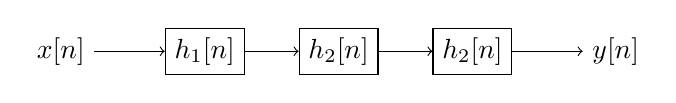
\begin{tikzpicture}
  \node[draw, minimum height=0.55cm] (A) at (0,0) {$h_1[n]$};
  \node[draw, minimum height=0.55cm] (B) at (1.7,0) {$h_2[n]$};
  \node[draw, minimum height=0.55cm] (C) at (3.4,0) {$h_2[n]$};
  \draw[->] (-1.4,0) node[left] {$x[n]$} -- (A.west);
  \draw[->] (A.east) -- (B.west);
  \draw[->] (B.east) -- (C.west);
  \draw[->] (C.east) -- (4.8,0) node[right] {$y[n]$};
\end{tikzpicture}
\end{center}
Cascade interconnection of three causal LTI systems

\noindent
\begin{minipage}[c]{0.4\linewidth}
$h_2[n] = u[n] - u[n-2]$

\medskip
Overall impulse response
\end{minipage}\hfill
\begin{minipage}[c]{0.56\linewidth}
\centering
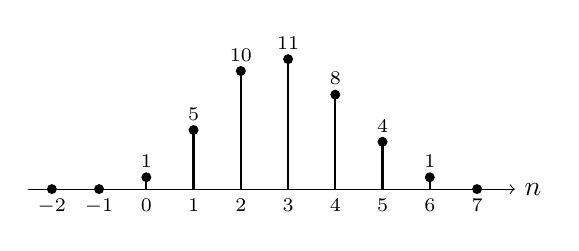
\begin{tikzpicture}[xscale=0.6, yscale=0.15]
  \draw[->] (-2.5,0) -- (7.8,0) node[right] {$n$};
  \foreach \x in {-2,-1,7} { \fill (\x,0) circle (3pt and 12pt); }
  \foreach \x/\y in {0/1,1/5,2/10,3/11,4/8,5/4,6/1} { \draw[thick] (\x,0) -- (\x,\y); \fill (\x,\y) circle (3pt and 12pt); \node[above] at (\x,\y) {\scriptsize $\y$}; }
  \foreach \x in {-2,...,7} { \node[below] at (\x,0) {\scriptsize $\x$}; }
\end{tikzpicture}
\end{minipage}

\medskip
$h_1[n] = ?$, \quad $x[n] = \delta[n] - \delta[n-1]$ için $y[n] = ?$
\end{ornek}
\begin{cozum}
\begin{center}
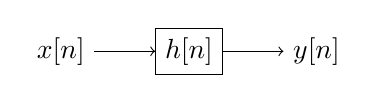
\begin{tikzpicture}
  \node[draw, minimum height=0.55cm] (H) at (0,0) {$h[n]$};
  \draw[->] (-1.2,0) node[left] {$x[n]$} -- (H.west);
  \draw[->] (H.east) -- (1.2,0) node[right] {$y[n]$};
\end{tikzpicture}
\end{center}
\[ h[n] = h_1[n] \ast h_2[n] \ast h_2[n] \]
Reminder: \ $u[n] = \displaystyle\sum_{k=0}^{\infty} \delta[n-k]$

\[ h_2[n] = \delta[n] + \delta[n-1] \qquad \text{\fcolorbox{kirmizikalem}{kagitrengi}{\color{turuncukalem}\small d[n]+d[n-1]}} \]
\begin{align*}
  h_2[n] \ast h_2[n] &= \delta[n] + 2\,\delta[n-1] + \delta[n-2] \\
  h_1[n] \ast h_2[n] \ast h_2[n] &= h_1[n] + 2h_1[n-1] + h_1[n-2] = h[n]
\end{align*}
\begin{align*}
  h[0] &= h_1[0] + 2\underset{\swarrow 0}{h_1[-1]} + \underset{\swarrow 0}{h_1[-2]} &&\rightarrow h_1[0] = 1 \\
  h[1] &= h_1[1] + 2h_1[0] + \underset{\swarrow 0}{h_1[-1]} &&\rightarrow h_1[1] = 3 \\
  h[2] &= h_1[2] + 2h_1[1] + h_1[0] &&\rightarrow h_1[2] = 3 \\
  & && \phantom{\rightarrow}\ h_1[3] = 2 \\
  & && \phantom{\rightarrow}\ h_1[4] = 1 \\
  & && \phantom{\rightarrow}\ h_1[5] = 0
\end{align*}
\[ y[n] = x[n] \ast h[n] = h[n] - h[n-1] \]
\end{cozum}

\end{document}
